\subsection{Afstand tussen twee punten in het vlak}
\noindent

Het vlak is voorzien van een Euclidisch assenstelsel.
Neem twee verschillende punten $P(a;b)$ en $Q(c;d)$ in het vlak.
We stellen de formule op waarmee je de afstand tussen $P$ en $Q$ (genoteerd $d(P;Q)$ uitdrukt met de Euclidische co\"ordinaten van $P$ en $Q$.

De loodrechte projecties van $P$ en $Q$ op de $x$-as noem je $P_1$ en $Q_1$.
De loodrechte projecties van $P$ en $Q$ op de $y$-as noem je $P_2$ en $Q_2$.
Deze punten hebben co\"ordinaten $P_1(a;0)$, $Q_1(c;0)$, $P_2(0;b)$ en $Q_2(0;d)$.

Als $b=d$ dan is de rechte $PQ$ evenwijdig met de $x$-as.
Als $a=c$ dan is de rechte $PQ$ evenwijdig met de $y$-as.
Stel dat de rechte $PQ$ noch horizontaal, noch verticaal is (dus $b\neq d$ en $a \neq c$).
Het snijpunt van de rechte door $P$ evenwijdig met de $y$-as met de rechte door $Q$ evenwijdig met de $x$-as noem je $R$.

\begin{center}
	\begin{tikzpicture}
	\draw[->] (-1,0)--(7,0) node[anchor=south,left,yshift=0.2cm]{$x$};
	\draw[->] (0,-1)--(0,6) node[anchor=south,left]{$y$};
	
	\tkzDefPoint(0,0){O}
	\tkzDefPoint(1,0){A}
	\tkzDefPoint(0,1){B}
	\tkzDefPoint(2,0){P1}
	\tkzDefPoint(6,0){Q1}
	\tkzDefPoint(0,2){Q2}
	\tkzDefPoint(0,5){P2}
	\tkzDefPoint(2,2){R}
	\tkzDefPoint(6,2){Q}
	\tkzDefPoint(2,5){P}
	
	\tkzDrawSegment[black!60!black,dotted](P1,R)
	\tkzDrawSegment[black!60!black,dotted](Q1,Q)
	\tkzDrawSegment[black!60!black,dotted](Q2,R)
	\tkzDrawSegment[black!60!black,dotted](P2,P)	
	\tkzDrawSegment[black!60!black](R,P)
	\tkzDrawSegment[black!60!black](Q,P)
	\tkzDrawSegment[black!60!black](R,Q)
	
	\tkzLabelPoint[below,xshift=-0.2cm](S){$0$}
	\tkzLabelPoint[below](A){$1$}
	\tkzLabelPoint[left](B){$1$}
	
	\tkzLabelPoint[below](P1){$a$}
	\tkzLabelPoint[below](Q1){$c$}
	\tkzLabelPoint[above](P1){$P_1$}
	\tkzLabelPoint[above](Q1){$Q_1$}
	
	\tkzLabelPoint[left](P2){$b$}
	\tkzLabelPoint[left](Q2){$d$}
	\tkzLabelPoint[right,yshift=0.2cm](Q2){$Q_2$}
	\tkzLabelPoint[right,yshift=0.2cm](P2){$P_2$}
	
	\tkzLabelPoint[above](P){$P$}
	\tkzLabelPoint[above,xshift=0.2cm](Q){$Q$}
	\tkzLabelPoint[above,xshift=0.2cm](R){$R$}
	
	\foreach \n in {O,A,B,P1,P2,Q1,Q2,P,Q,R}
	\node at (\n)[circle,fill,inner sep=1.5pt]{};
	
	\end{tikzpicture}
\end{center}

%\gewonefiguur{height=5cm}{4_opp_inhoud_an_meetk/inputs/AMTekst3Fig1}

%\begin{figure}[!htb]
%\begin{center}
%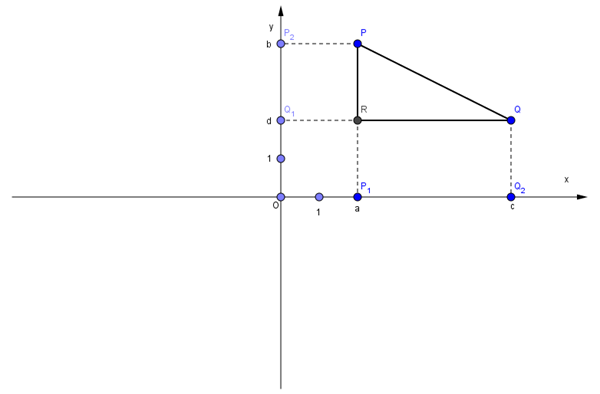
\includegraphics[width=.7\linewidth]{4_opp_inhoud_an_meetk/inputs/AMTekst3Fig1}
%\caption{}
%\label{fig4.2.3_fig1}
%\end{center}
%\end{figure}

In de rechthoekige driehoek $PQR$ geeft de Stelling van Pythagoras:
\[
\vert PQ \vert ^2= \vert PR \vert ^2+ \vert QR \vert ^2 \text {.}
\]
Er geldt $\vert PR \vert = \vert Q_2P_2 \vert = d(Q_2;P_2)=\vert b-d \vert$.
Dit laatste is waar omdat $b$ en $d$ abscissen zijn van $P_2$ en $Q_2$ op de geijkte $y$-as die overeenkomt met de lengte-eenheid.
Er geldt ook $\vert QR \vert = \vert P_1Q_1 \vert = d(P_1;Q_1)=\vert a-c \vert$.
Invullen in de Stelling van Pythagoras geeft
\[
\vert PQ \vert ^2=(b-d)^2+(a-c)^2 \text{ .}
\]
Hieruit vind je
\[
d(P;Q)=\sqrt{(b-d)^2+(a-c)^2} \text { .}
\]\vspace{2mm}

De formule geldt ook als de rechte $PQ$ wel evenwijdig is met de $x$-as of de $y$-as.
\begin{itemize}
\item De rechte $PQ$ is horizontaal, dus $b=d$.

\begin{center}
	\begin{tikzpicture}
	\draw[->] (-1,0)--(6,0) node[anchor=south,left,yshift=0.2cm]{$x$};
	\draw[->] (0,-1)--(0,6) node[anchor=south,left]{$y$};
	
	\tkzDefPoint(0,0){O}
	\tkzDefPoint(1,0){A}
	\tkzDefPoint(0,1){B}
	\tkzDefPoint(2,0){P1}
	\tkzDefPoint(5,0){Q1}
	\tkzDefPoint(0,2){Q2}
	\tkzDefPoint(5,2){Q}
	\tkzDefPoint(2,2){P}
	
	\tkzDrawSegment[black!60!black,dotted](P1,P)
	\tkzDrawSegment[black!60!black,dotted](Q1,Q)
	\tkzDrawSegment[black!60!black,dotted](Q2,P)
	\tkzDrawSegment[black!60!black](Q,P)
	
	\tkzLabelPoint[below,xshift=-0.2cm](S){$0$}
	\tkzLabelPoint[below](A){$1$}
	\tkzLabelPoint[left](B){$1$}
	
	\tkzLabelPoint[below](P1){$a$}
	\tkzLabelPoint[below](Q1){$c$}
	\tkzLabelPoint[above](P1){$P_1$}
	\tkzLabelPoint[above](Q1){$Q_1$}
	
	\tkzLabelPoint[left](Q2){$b=d$}
	\tkzLabelPoint[right,yshift=0.2cm](Q2){$P_2=Q_2$}
	
	\tkzLabelPoint[above](P){$P$}
	\tkzLabelPoint[above](Q){$Q$}
	
	\foreach \n in {O,A,B,P1,P2,Q1,P,Q,R}
	\node at (\n)[circle,fill,inner sep=1.5pt]{};
	
	\end{tikzpicture}
\end{center}

%\gewonefiguur{width=.7\linewidth}{4_opp_inhoud_an_meetk/inputs/AMTekst3Fig2}

%\begin{figure}[!htb]
%\begin{center}
%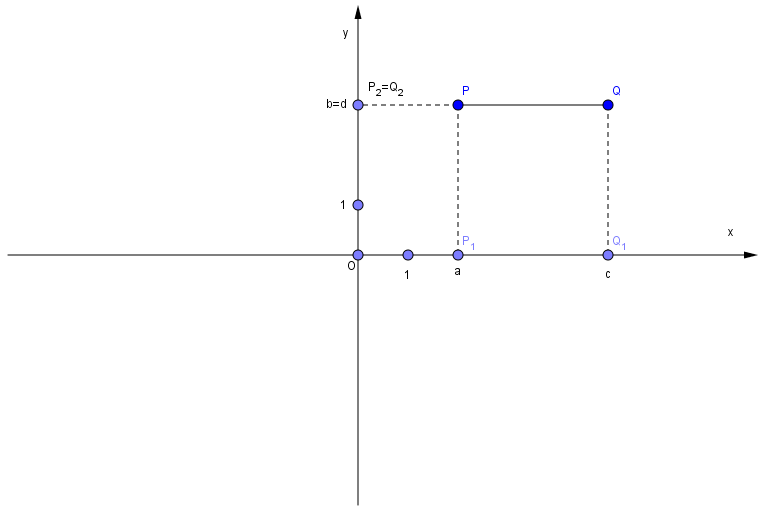
\includegraphics[width=.7\linewidth]{4_opp_inhoud_an_meetk/inputs/AMTekst3Fig2}
%\caption{}
%\label{fig4.2.3_fig2}
%\end{center}
%\end{figure}

\[
d(P;Q)=d(P_1;Q_1)=\vert c-a \vert \text { en } \sqrt { (b-d)^2+(a-c)^2 }=\vert c-a \vert
\]
\item De rechte $PQ$ is verticaal, dus $a=c$.

\begin{center}
	\begin{tikzpicture}
	\draw[->] (-1,0)--(7,0) node[anchor=south,left,yshift=0.2cm]{$x$};
	\draw[->] (0,-4)--(0,6) node[anchor=south,left]{$y$};
	
	\tkzDefPoint(0,0){O}
	\tkzDefPoint(1,0){A}
	\tkzDefPoint(0,1){B}
	\tkzDefPoint(2,0){P1}
	\tkzDefPoint(0,-3){Q2}
	\tkzDefPoint(0,5){P2}
	\tkzDefPoint(2,-3){Q}
	\tkzDefPoint(2,5){P}
	
	\tkzDrawSegment[black!60!black,dotted](Q2,Q)
	\tkzDrawSegment[black!60!black,dotted](P2,P)	
	\tkzDrawSegment[black!60!black](Q,P)
	
	\tkzLabelPoint[below,xshift=-0.2cm](S){$0$}
	\tkzLabelPoint[below](A){$1$}
	\tkzLabelPoint[left](B){$1$}
	
	\tkzLabelPoint[below,xshift=0.2cm](P1){$a=c$}
	\tkzLabelPoint[above,xshift=0.2cm](P1){$P_1=Q_1$}
	
	\tkzLabelPoint[left](P2){$b$}
	\tkzLabelPoint[left](Q2){$d$}
	\tkzLabelPoint[right,yshift=0.2cm](Q2){$Q_2$}
	\tkzLabelPoint[right,yshift=0.2cm](P2){$P_2$}
	
	\tkzLabelPoint[above](P){$P$}
	\tkzLabelPoint[above,xshift=0.2cm](Q){$Q$}
	
	\foreach \n in {O,A,B,P1,P2,Q2,P,Q}
	\node at (\n)[circle,fill,inner sep=1.5pt]{};
	
	\end{tikzpicture}
\end{center}

%\gewonefiguur{height=5cm}{4_opp_inhoud_an_meetk/inputs/AMTekst3Fig3}
%\begin{figure}[!htb]
%\begin{center}
%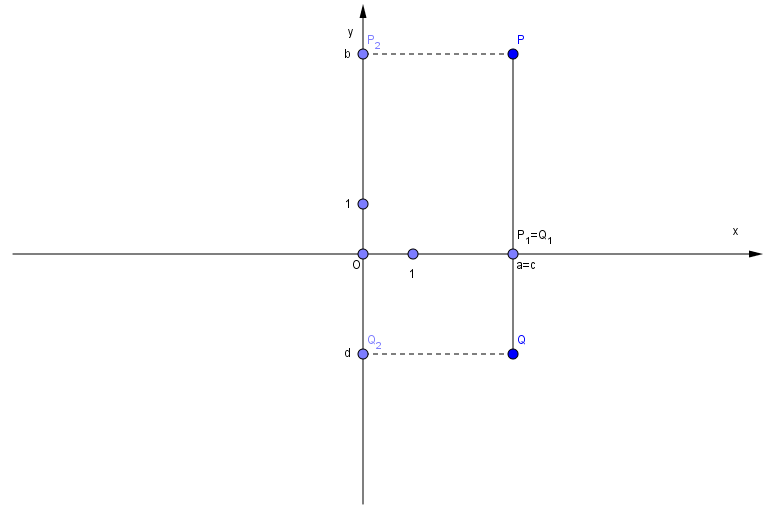
\includegraphics[width=.7\linewidth]{4_opp_inhoud_an_meetk/inputs/AMTekst3Fig3}
%\caption{}
%\label{fig4.2.3_fig3}
%\end{center}
%\end{figure}
\[
d(P;Q)=d(P_2;Q_2)=\vert d-b \vert \text { en } \sqrt { (b-d)^2+(a-c)^2 }=\vert b-d \vert
\]
\end{itemize}\vspace{2mm}

\newpage

\begin{voorbeeld}
Bereken de afstand tussen $P(2;-3)$ en $Q(-5;-2)$.

\begin{center}
	\begin{tikzpicture}
	\draw[->] (-6,0)--(4,0) node[anchor=south,left,yshift=0.2cm]{$x$};
	\draw[->] (0,-4)--(0,2) node[anchor=south,left]{$y$};
	
	\tkzDefPoint(0,0){O}
	\tkzDefPoint(1,0){A}
	\tkzDefPoint(0,1){B}
	\tkzDefPoint(2,0){P1}
	\tkzDefPoint(-5,0){Q1}
	\tkzDefPoint(0,-2){Q2}
	\tkzDefPoint(0,-3){P2}
	\tkzDefPoint(2,-3){P}
	\tkzDefPoint(-5,-2){Q}
	
	\tkzDrawSegment[black!60!black,dotted](P1,P)
	\tkzDrawSegment[black!60!black,dotted](P2,P)
	\tkzDrawSegment[black!60!black,dotted](Q1,Q)
	\tkzDrawSegment[black!60!black,dotted](Q2,Q)
	
	\tkzLabelPoint[below,xshift=-0.2cm](S){$0$}
	\tkzLabelPoint[below](A){$1$}
	\tkzLabelPoint[left](B){$1$}
	
	\tkzLabelPoint[below](P1){$2$}
	\tkzLabelPoint[below](Q1){$-2$}
	
	\tkzLabelPoint[left](P2){$-3$}
	\tkzLabelPoint[right](Q2){$-2$}
	
	\tkzLabelPoint[right](P){$P$}
	\tkzLabelPoint[left](Q){$Q$}
	
	\foreach \n in {O,A,B,P1,P2,Q1,P,Q,Q2}
	\node at (\n)[circle,fill,inner sep=1.5pt]{};
	
	\end{tikzpicture}
\end{center}

%\gewonefiguur{height=5cm}{4_opp_inhoud_an_meetk/inputs/AMTekst3Fig4}

%\begin{figure}[!htb]
%\begin{center}
%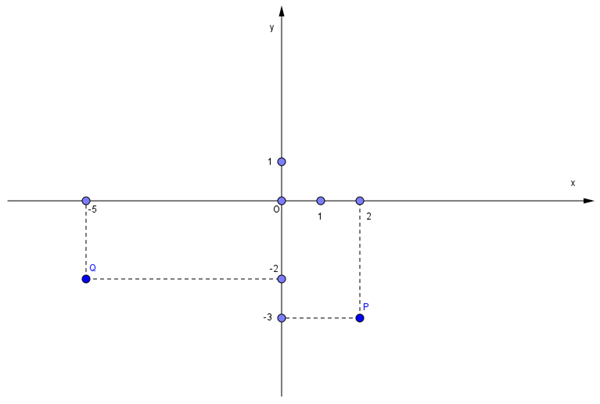
\includegraphics[width=.7\linewidth]{4_opp_inhoud_an_meetk/inputs/AMTekst3Fig4}
%\caption{Voorbeeld 1.}
%\label{fig4.2.3_fig4}
%\end{center}
%\end{figure}
\[
d(P;Q)=\sqrt{(-5-2)^2+(-2-(-3))^2}=\sqrt{50}
\]\vspace{3mm}

%Voor de makers: volgend voorbeeld tekening tonen en daarnaast berekeningen met topcamera.
\end{voorbeeld}

\begin{voorbeeld}
Gegeven zijn de punten $P(-2;5)$ en $Q(3;-1)$.
Wat zijn de co\"ordinaten van het punt $R$ met $x$-co\"ordinaat gelijk aan 2 dat even ver van $P$ als van $Q$ ligt?

\begin{center}
	\begin{tikzpicture}
	\draw[->] (-6,0)--(4,0) node[anchor=south,left,yshift=0.2cm]{$x$};
	\draw[->] (0,-2)--(0,7) node[anchor=south,left]{$y$};
	\draw[-] (2,-2)--(2,7);
	
	\tkzDefPoint(0,0){O}
	\tkzDefPoint(1,0){A}
	\tkzDefPoint(0,1){B}
	\tkzDefPoint(-2,0){P1}
	\tkzDefPoint(3,0){Q1}
	\tkzDefPoint(0,-1){Q2}
	\tkzDefPoint(0,5){P2}
	\tkzDefPoint(-2,5){P}
	\tkzDefPoint(3,-1){Q}
	
	\tkzDrawSegment[black!60!black,dotted](P1,P)
	\tkzDrawSegment[black!60!black,dotted](P2,P)
	\tkzDrawSegment[black!60!black,dotted](Q1,Q)
	\tkzDrawSegment[black!60!black,dotted](Q2,Q)
	
	\tkzLabelPoint[below,xshift=-0.2cm](S){$0$}
	\tkzLabelPoint[below](A){$1$}
	\tkzLabelPoint[left](B){$1$}
	
	\tkzLabelPoint[below](P1){$-2$}
	\tkzLabelPoint[below](Q1){$3$}
	
	\tkzLabelPoint[right](P2){$5$}
	\tkzLabelPoint[left](Q2){$-1$}
	
	\tkzLabelPoint[right](P){$P$}
	\tkzLabelPoint[left](Q){$Q$}
	
	\foreach \n in {O,A,B,P1,P2,Q1,P,Q,Q2}
	\node at (\n)[circle,fill,inner sep=1.5pt]{};
	
	\end{tikzpicture}
\end{center}

%\gewonefiguur{height=5cm}{4_opp_inhoud_an_meetk/inputs/AMTekst3Fig5}
%\begin{figure}[!htb]
%\begin{center}
%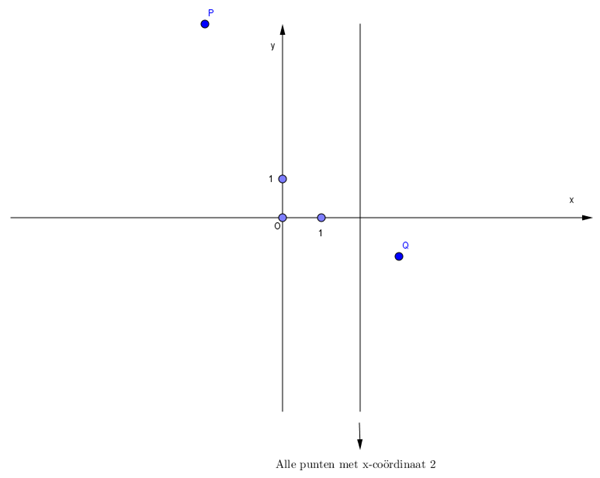
\includegraphics[width=.7\linewidth]{4_opp_inhoud_an_meetk/inputs/AMTekst3Fig5}
%\caption{Voorbeeld 2.}
%\label{fig4.2.3_fig5}
%\end{center}
%\end{figure}

$R$ heeft co\"ordinaten $(2;y)$.
We zoeken $y$ zodat $d(R;P)=d(R;Q)$.
\[
d(R;P)=\sqrt{(-2-2)^2+(y-5)^2}=\sqrt{16+(y-5)^2}
\]
\[
d(R;Q)=\sqrt{(3-2)^2+(y-(-1))^2}=\sqrt{1+(y+1)^2}
\]
Hieruit volgt dat $d(R;P)=d(R;Q)$ als en alleen als
\[
16+(y-5)^2=1+(y+1)^2
\]
Uitwerken van de kwadraten geeft
\[
16+y^2-10y+25=1+y^2+2y+1 \text { dus } 12y=39 \text { .}
\]
Het punt $R$ heeft co\"ordinaten $(2;\frac{39}{12})$.
\end{voorbeeld}